% Advisor report; provenance and reproduction are in README.md / SOURCES.md.
% WBR advisor progress report -- evidence snapshot 2026-10-14.
% Build: latexmk -xelatex main.tex   (see README.md)
% Content sources and number provenance: SOURCES.md.
% Historical Pi measurements are labeled MEASURED; calculations, assumptions,
% published comparisons, plans and OPEN qualification remain distinct.
\documentclass[aspectratio=169,12pt,t]{beamer}

% Speaker notes: uncomment ONE line to see them.
% \setbeameroption{show notes on second screen=right}  % dual-screen (pdfpc)
% \setbeameroption{show only notes}                     % notes handout

\usetheme[progressbar=none, sectionpage=none]{moloch}
% A 208 x 117 mm canvas retains 16:9 and the actual 12pt class fonts.
% Long owner-approved sentences fit without frame scaling or reduced fonts.
\geometry{paperwidth=208mm,paperheight=117mm}

% ---------- fonts ----------
\usepackage{fontspec}
\setsansfont{Avenir Next}[BoldFont={Avenir Next Demi Bold}]
\setmonofont{Menlo}[Scale=1.0]
\newcommand{\captiontype}{\small}

% ---------- palette ----------
\definecolor{navy}{HTML}{1F3A5F}
\definecolor{teal}{HTML}{2A9D8F}
\definecolor{fault}{HTML}{E76F51}
\definecolor{paper}{HTML}{FAFAF7}
\definecolor{ink}{HTML}{22262B}
\definecolor{muted}{HTML}{6B7280}
\definecolor{rule}{HTML}{D6D9DE}

\setbeamercolor{normal text}{fg=ink, bg=paper}
\setbeamercolor{frametitle}{fg=paper, bg=navy}
\setbeamercolor{progress bar}{fg=teal, bg=rule}
\setbeamercolor{alerted text}{fg=fault}
\setbeamercolor{example text}{fg=teal}
\setbeamercolor{structure}{fg=navy}
\setbeamercolor{title separator}{fg=teal}
\setbeamercolor{footline}{fg=muted}
% Beamer otherwise inherits the fault/alert color for in-slide citations.
\setbeamercolor{bibliography entry author}{fg=navy}
\setbeamercolor{bibliography entry title}{fg=ink}
\setbeamercolor{bibliography entry location}{fg=muted}
\setbeamercolor{bibliography entry note}{fg=muted}
\setbeamercolor{block title}{fg=paper, bg=navy}
\setbeamercolor{block body}{bg=navy!6}
\setbeamerfont{frametitle}{size=\large, series=\bfseries}
\setbeamertemplate{frametitle}{\nointerlineskip\begin{beamercolorbox}[wd=\paperwidth,sep=2mm,leftskip=4mm]{frametitle}\usebeamerfont{frametitle}\insertframetitle\strut\end{beamercolorbox}}
\setbeamertemplate{itemize items}{\color{teal}\rule[0.25ex]{0.45em}{0.45em}}
\setbeamertemplate{bibliography item}[text]
\setbeamertemplate{page number in head/foot}[totalframenumber]
\hypersetup{colorlinks=true, linkcolor=navy, urlcolor=navy, citecolor=navy}
% Keep the appendix bookmark free of Beamer translation commands.
\pdfstringdefDisableCommands{\def\translate#1{#1}}

\setbeamertemplate{itemize subitem}{\color{muted}--}

% ---------- packages ----------
\usepackage{tikz}
\usetikzlibrary{arrows.meta, positioning, automata, calc, shapes.geometric, fit, backgrounds, decorations.pathreplacing}
\usepackage{booktabs}
\usepackage{array}
\newcolumntype{L}[1]{>{\raggedright\arraybackslash}p{#1}}
\usepackage{amsmath}
\usepackage{siunitx}
\sisetup{detect-all}

% ---------- helpers ----------
\newcommand{\muted}[1]{{\color{muted}#1}}

% \slideimg[<max height>]{<width>}{<V-id>}{<caption for placeholder>}
% Shows images/<V-id>.jpg or .png if present, otherwise a labelled gray box of the same size.
\newcommand{\slideimg}[4][0.64\textheight]{%
  \IfFileExists{images/#3.jpg}{%
    \includegraphics[width=#2, height=#1, keepaspectratio]{images/#3.jpg}%
  }{\IfFileExists{images/#3.png}{%
    \includegraphics[width=#2, height=#1, keepaspectratio]{images/#3.png}%
  }{%
    \begin{tikzpicture}
      \node[draw=rule, fill=black!6, rounded corners=2pt, minimum width=\dimexpr#2-1pt\relax, outer sep=0pt,
            minimum height=#1, align=center, text width=\dimexpr#2-8mm\relax, font=\small, text=muted]
        {\textbf{#3}\\[2pt]#4\\[2pt]\small Illustration pending};
    \end{tikzpicture}%
  }}%
}

\tikzset{
  box/.style={draw=navy, fill=white, rounded corners=2pt, align=center, font=\small,
              minimum height=7mm, inner sep=3pt},
  flow/.style={-{Stealth[length=2mm]}, thick, color=navy},
  faultflow/.style={-{Stealth[length=2mm]}, thick, color=fault},
  lbl/.style={font=\small, color=ink, fill=paper, inner sep=1pt},
}

% Only the page number appears in the footer.
\setbeamerfont{footline}{size=\small}
\setbeamertemplate{footline}{\hbox{\begin{beamercolorbox}[wd=\paperwidth,ht=4mm,dp=1mm,rightskip=6mm]{footline}\hfill\insertframenumber/\inserttotalframenumber\end{beamercolorbox}}}
\AtBeginSection{\begin{frame}[c]\centering{\Huge\bfseries\color{navy}\thesection. \insertsectionhead\par}\end{frame}}
\setbeamertemplate{navigation symbols}{}
\setbeamersize{text margin left=6mm,text margin right=6mm}
\setlength{\tabcolsep}{4pt}
\renewcommand{\arraystretch}{1.02}
\title{WBR Perception: Progress Report}
\subtitle{Known baseline; first camera diagnostics}
\author{}
\institute{}
\date{14 October 2026}


\newcounter{slidefigure}
\newcommand{\figcap}[1]{\par\smallskip{\centering\captiontype\color{muted}\refstepcounter{slidefigure}Figure \theslidefigure: #1\par}}
\newcommand{\figagain}[1]{\par\smallskip{\centering\captiontype\color{muted}Figure~\ref{fig:#1}: \csuse{caption#1}\par}}
\setbeamerfont{bibliography entry author}{size=\normalsize}
\setbeamerfont{bibliography entry title}{size=\normalsize}
\setbeamerfont{bibliography entry location}{size=\normalsize}
\setbeamerfont{bibliography entry note}{size=\normalsize}
\setlength{\emergencystretch}{2em}
\setbeamerfont{normal text}{size=\normalsize}
\setbeamerfont{itemize/enumerate body}{size=\normalsize}
\setbeamerfont{itemize/enumerate subbody}{size=\normalsize}
\linespread{1.12}
\AtBeginDocument{\setlength{\leftmargini}{1.1em}\setlength{\leftmarginii}{1.2em}\setlength{\labelsep}{.35em}}
\newcommand{\namedcap}[2]{\figcap{#2}}
% Apply spacing after Beamer has created each list (including nested lists).
\usepackage{etoolbox}
\makeatletter
\apptocmd{\itemize}{\ifnum\@itemdepth=1\setlength{\itemsep}{.55em}\else\setlength{\itemsep}{.25em}\fi\setlength{\parsep}{0pt}\setlength{\parskip}{0pt}\setlength{\topsep}{0pt}}{}{}
\makeatother
\newsavebox{\figurebox}
\newcommand{\fig}[3][.48\textheight]{%
  \ifcsdef{diagram#2}{\sbox{\figurebox}{\csuse{diagram#2}}}{%
    \sbox{\figurebox}{\includegraphics[width=\linewidth,height=#1,keepaspectratio]{images/#2.jpg}}}%
  \par\centering\begin{minipage}{\wd\figurebox}\centering
  \usebox{\figurebox}%
  \ifcsdef{assetcaption#2}{\csuse{assetcaption#2}}{%
    \csgdef{assetcaption#2}{\repeatassetcap{#2}}%
    \csgdef{assettext#2}{#3}\figcap{#3}%
    \csxdef{assetnumber#2}{\theslidefigure}}\end{minipage}\par}
\newcommand{\repeatassetcap}[1]{\par\smallskip{\centering\captiontype\color{muted}%
  \begingroup\renewcommand{\label}[1]{}Figure \csuse{assetnumber#1}: \csuse{assettext#1}\par\endgroup}}
\makeatletter
\newcommand{\takeaway}[1]{\global\beamer@framebottomskip=0pt\par\medskip\begin{beamercolorbox}[wd=\linewidth,sep=0pt]{block body}%
  \begin{tabular}{@{}!{\color{teal}\vrule width 3pt}p{\dimexpr\linewidth-22pt\relax}@{}}\normalsize\strut #1\strut\end{tabular}%
  \end{beamercolorbox}\par}
\makeatother


% Course additions retain the approved palette, canvas, type and figure system.
\newcommand{\evidence}[1]{{\small\bfseries\color{teal!70!black}#1}\par\medskip}
\newcommand{\coursefigure}[3]{\begin{minipage}{\linewidth}\centering#2\figcap{\label{fig:#1}#3}\end{minipage}}



\newcommand{\deckitems}[1]{\begin{itemize}#1\end{itemize}}
\newcommand{\deckflow}[1]{\begin{tikzpicture}[node distance=9mm]
\foreach \txt [count=\i] in {#1}{\node[box,font=\normalsize,text width=33mm,minimum height=14mm] (n\i) at ({mod(\i-1,4)*4.7},{-floor((\i-1)/4)*2.4}) {\txt};}
\end{tikzpicture}}


\newcommand{\src}[1]{\note{Source: #1}}% sources moved to speaker notes (owner request 2026-10-14)
\newcommand{\epath}[1]{{\small\ttfamily\detokenize{#1}}}
\begin{document}
\raggedright

% 1
\begin{frame}[c]\relax
{\huge\bfseries\color{navy}WBR Perception\par}
{\Large\color{teal}Progress report · 14 October 2026\par}
\medskip{\color{teal}\hrule height .6pt}\medskip
\begin{columns}[c,onlytextwidth]
\begin{column}{.54\textwidth}
\Large Known baseline; first\par camera diagnostics\par\bigskip
\normalsize Pi 5 · D435i · ORB-SLAM3\par\medskip
\textbf{Accuracy evidence is encouraging.}\par
Physical qualification remains OPEN.
\end{column}
\begin{column}{.42\textwidth}
\slideimg[.43\textheight]{\linewidth}{P04}{D435i stereo camera}
\par\small\color{muted}Sensor illustration; no validation claim.
\end{column}\end{columns}
\note{About 15 minutes for slides 1--17; four backups and references follow. All results are historical evidence read on the Mac, not fresh experiments. No gate is promoted to PASS. The owner generates any new raster illustration; this report only reuses P04.}
\end{frame}

% 2
\begin{frame}{Goal: useful navigation without coupling balance to Linux}
\evidence{PLANNED}
\Large A wheel-biped robot needs scene-relative motion for navigation.\par\bigskip
\normalsize\deckitems{
\item Pi 5 estimates motion from stereo images and inertial data.
\item STM32H7 owns balance, hard-real-time control and motor safety.
\item Perception failure must remove optional navigation input safely.}
\vfill\takeaway{Qualify perception while preserving the controller ownership boundary.}
\src{AGENTS.md; docs/ARCHITECTURE.md}
\note{WBR means wheel-biped robot: torso, two articulated legs, one wheel at each foot. The boundary is a design requirement, not a tested robot-safety result. No mechanical drawing is claimed.}
\end{frame}

% 3
\begin{frame}{Ownership: the Pi provides an optional reference}
\evidence{PLANNED / OPEN integration}
\centering
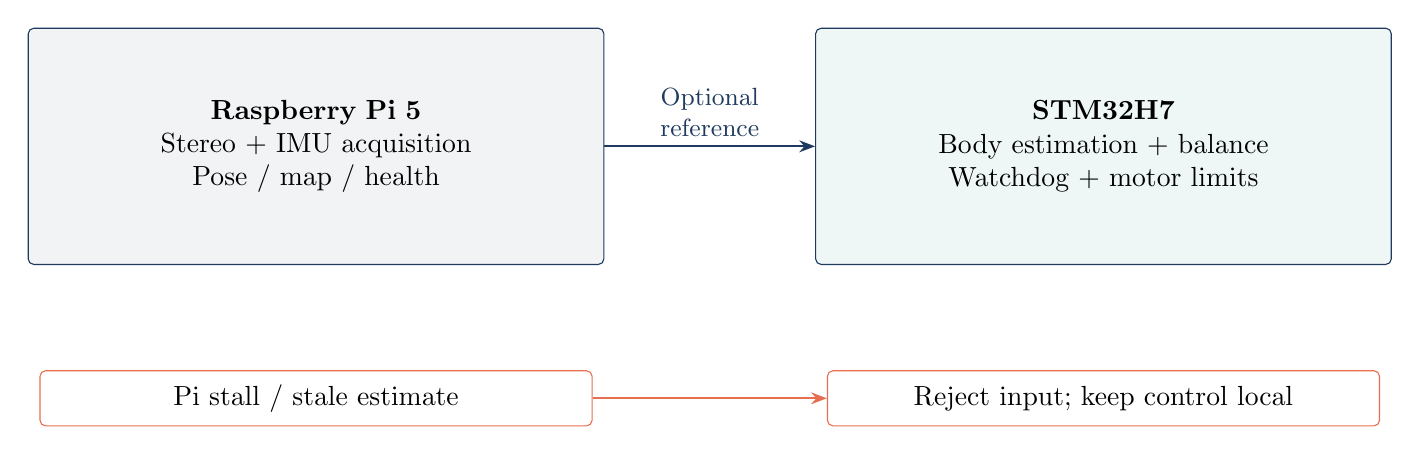
\begin{tikzpicture}
\node[box,text width=71mm,minimum height=30mm,font=\normalsize,fill=navy!6] (pi) at (0,0) {\textbf{Raspberry Pi 5}\\Stereo + IMU acquisition\\Pose / map / health};
\node[box,text width=71mm,minimum height=30mm,font=\normalsize,fill=teal!8] (mcu) at (10,0) {\textbf{STM32H7}\\Body estimation + balance\\Watchdog + motor limits};
\draw[flow] (pi.east)--node[above,align=center,font=\small]{Optional\\reference}(mcu.west);
\node[box,text width=68mm,draw=fault,font=\normalsize] (fail) at (0,-3.2) {Pi stall / stale estimate};
\node[box,text width=68mm,draw=fault,font=\normalsize] (safe) at (10,-3.2) {Reject input; keep control local};
\draw[faultflow] (fail.east)--(safe.west);
\end{tikzpicture}
\vfill\takeaway{Receiver health semantics and physical fault tests are still future gates.}
\src{AGENTS.md; docs/ARCHITECTURE.md}
\note{This is the existing ownership model, not a new node graph or public message proposal. Transport, clock relation, age thresholds and fallback bounds require review in N6/N7. No motor or controller test was performed.}
\end{frame}

% 4
\begin{frame}{Data path: two ways to read the camera}
\evidence{MEASURED recording / OPEN replay / PLANNED ROS 2}
\centering
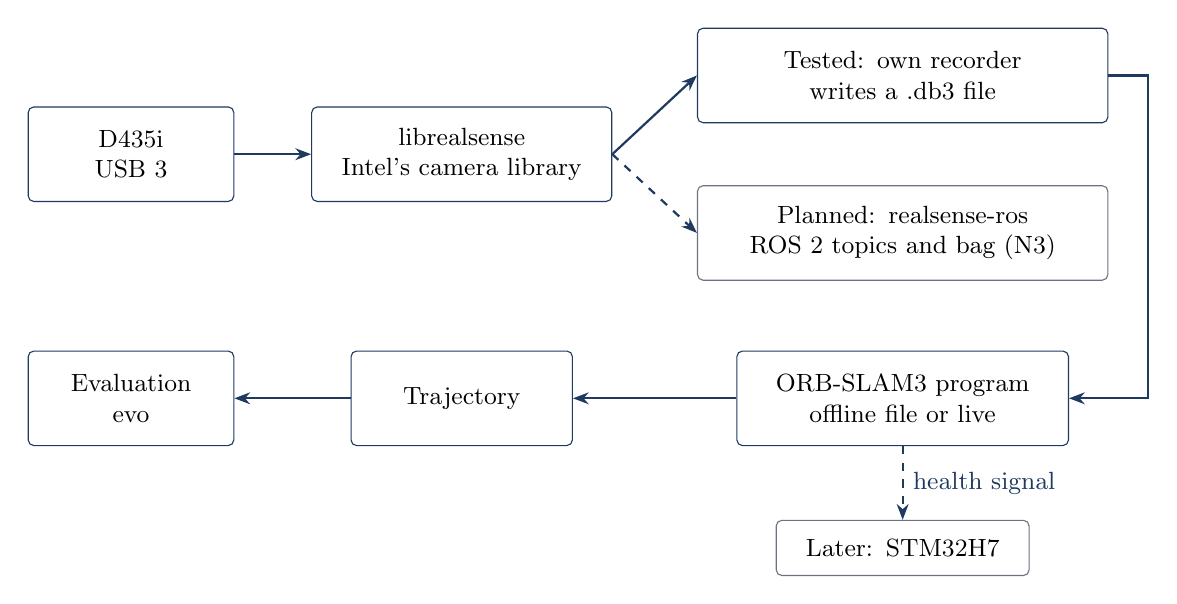
\begin{tikzpicture}[font=\normalsize]
\node[box,text width=24mm,minimum height=12mm] (d) at (0,0) {D435i\\USB 3};
\node[box,text width=36mm,minimum height=12mm] (sdk) at (4.2,0) {librealsense\\\small Intel's camera library};
\node[box,text width=50mm,minimum height=12mm] (rec) at (9.8,1.0) {Tested: own recorder\\\small writes a .db3 file};
\node[box,draw=muted,text width=50mm,minimum height=12mm] (ros) at (9.8,-1.0) {Planned: realsense-ros\\\small ROS 2 topics and bag (N3)};
\node[box,text width=40mm,minimum height=12mm] (orb) at (9.8,-3.1) {ORB-SLAM3 program\\\small offline file or live};
\node[box,text width=26mm,minimum height=12mm] (traj) at (4.2,-3.1) {Trajectory};
\node[box,text width=24mm,minimum height=12mm] (eval) at (0,-3.1) {Evaluation\\\small evo};
\draw[flow] (d)--(sdk);\draw[flow] (sdk.east)--(rec.west);\draw[flow,dashed] (sdk.east)--(ros.west);
\draw[flow] (rec.east)--++(0.5,0)|-(orb.east);
\draw[flow] (orb)--(traj);\draw[flow] (traj)--(eval);
\node[box,draw=muted,text width=30mm] (stm) at (9.8,-5.0) {Later: STM32H7};
\draw[flow,dashed] (orb)--node[right,font=\small]{health signal}(stm);
\end{tikzpicture}
\vfill\takeaway{Today's two programs use librealsense directly, without ROS 2; the ROS 2 path (N3) is still required.}
\src{Session facts §E; N4B prep/n4b\_plan.md; 14 October addendum §§2--5}
\note{librealsense is Intel's RealSense SDK: the C++ library that talks to the camera over USB. The recorder and the D435i ORB-SLAM3 program built on 2026-10-13 use it directly (no ROS 2 node, no topics); the program reads either the recorded .db3 file (offline, N4B) or the camera (live, N4C). Short recorder tests succeeded; offline ORB-SLAM3 crashed on its first frame. Patch 4 rebuild and replay remain pending. Live ORB-SLAM3 is unverified. The ROS 2 path (realsense-ros publishing topics, recorded with rosbag2) is the separate N3 gate and remains required for the robot integration.}
\end{frame}

% 5
\begin{frame}{Method: each gate needs artifacts and acceptance}
\evidence{PLANNED / OPEN}
\centering
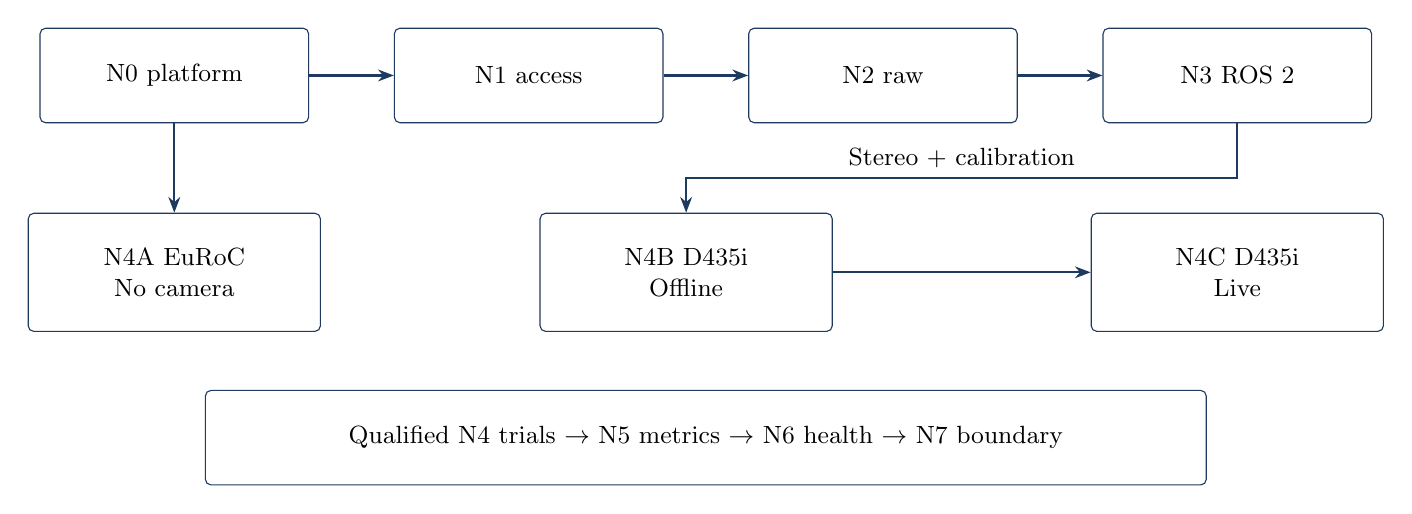
\begin{tikzpicture}[font=\normalsize]
\foreach \x/\id/\txt in {0/a/N0 platform,4.5/b/N1 access,9/c/N2 raw,13.5/d/N3 ROS 2}{\node[box,text width=32mm,minimum height=12mm] (\id) at (\x,0) {\txt};}
\draw[flow](a)--(b);\draw[flow](b)--(c);\draw[flow](c)--(d);
\node[box,text width=35mm,minimum height=15mm] (ea) at (0,-2.5) {N4A EuRoC\\No camera};
\node[box,text width=35mm,minimum height=15mm] (eb) at (6.5,-2.5) {N4B D435i\\Offline};
\node[box,text width=35mm,minimum height=15mm] (ec) at (13.5,-2.5) {N4C D435i\\Live};
\draw[flow](a)--(ea);\draw[flow](d.south)--(13.5,-1.3)--(6.5,-1.3)--(eb.north);
\node[font=\small,anchor=south] at (10,-1.3) {Stereo + calibration};
\draw[flow](eb)--(ec);
\node[box,text width=125mm,minimum height=12mm] at (6.75,-4.6) {Qualified N4 trials $\rightarrow$ N5 metrics $\rightarrow$ N6 health $\rightarrow$ N7 boundary};
\end{tikzpicture}
\vfill\takeaway{Build success, plausible trajectories and historical receipts do not imply gate PASS.}
\note{N4A needs an eligible N0 and separate execution authorization; it does not depend on camera gates. N4B requires N3, a reviewed stereo extension and accepted calibration. N4C renews input qualification under stereo load. Gate definitions follow the course, sections 4.1--4.14; thresholds remain unchanged. N5--N7 await qualified inputs and reviewed bounds.}
\end{frame}

% 6
\begin{frame}{Gate status: the active unit needs fresh physical evidence}
\evidence{OPEN · as of 14 October 2026}
\begin{tabular}{@{}L{45mm}L{140mm}@{}}\toprule
\textbf{Gate} & \textbf{Current status}\\\midrule
N0 platform & OPEN: loaded power unstable\\[8pt]
N1 access & OPEN: new unit; prior clock stop\\[8pt]
N2 raw & OPEN: new-unit soak missing\\[8pt]
N3 ROS 2 & OPEN: record/replay unqualified\\\bottomrule
\end{tabular}
\vfill\takeaway{Old-unit N1/N2 and calibration receipts do not transfer to the new D435i.}
\note{Session facts supersede historical inventory drafts in PROJECT_STATE. New unit SDK 317422076650; USB descriptor 327743061057. Clock was corrected later but fresh sealed N1 evidence is still missing. N2 exact profile remains IR1 640x480 Y8/15, gyro 200, accel 100; mandatory 300-second soak unchanged.}
\end{frame}

% 7
\begin{frame}{Gate status: measured accuracy; adaptation still OPEN}
\evidence{OPEN / PLANNED · as of 14 October 2026}
\begin{tabular}{@{}L{45mm}L{140mm}@{}}\toprule
\textbf{Gate} & \textbf{Current status}\\\midrule
N4A EuRoC & OPEN: three runs; timing invalid\\[7pt]
N4B offline & OPEN: first-frame crash; rebuild pending\\[7pt]
N4C live & OPEN: built; never camera-run\\[7pt]
N5 metrics & PLANNED: full campaign pending\\[7pt]
N6 health & PLANNED: semantics/fixtures\\[7pt]
N7 boundary & PLANNED: bench review/tests\\\bottomrule
\end{tabular}
\note{Sources remain in notes. Addendum §5 supersedes the earlier built-not-run N4B status. N4A has preliminary ATE metrics, not qualified N5 campaign evidence. The latest build/run status comes from the authoritative session summary; earlier prep receipts describe Mac-only work and must not be mistaken for subsequent Pi runtime receipts.}
\end{frame}

% 8
\begin{frame}{Since the previous report: a runnable native baseline}
\evidence{MEASURED}
\begin{tabular}{@{}L{43mm}L{140mm}@{}}\toprule
\textbf{Changed} & \textbf{Consequence}\\\midrule
New D435i unit & Camera serial \texttt{317422076650}; USB serial \texttt{327743061057}.\newline Renew physical input and calibration evidence.\\[12pt]
Active Pi 5 & 8 GB board; measured 7.8 GiB RAM; same 32 GB microSD.\newline Same 5 V / 3 A supply: under-voltage still present.\\[12pt]
Native ORB-SLAM3 & Three build patches; patch 4 applied, rebuild pending.\newline Isolated Pi copy; historical EuRoC example/settings unchanged.\\\bottomrule
\end{tabular}
\vfill\takeaway{The algorithm path now runs; the hardware change restarts camera qualification.}
\src{Session facts §A--C; N4A/provenance.txt; 14 October addendum §§1,5}
\note{New unit firmware 5.17.3.10, BMI085, USB 5000 Mbps. SDK, ASIC, firmware-update ID and descriptor serial are separate fields; USB/ASIC association here is reported evidence, not a general identity rule. Three patches: C++17/drop march native, disable failing Sophus tests, bool increment replaced with true. Pi build around 71 min at j2 with 4 GB temporary swap. Addendum §1 measures 7.8 GiB on the active 8 GB Pi. Patch 4 rebuild was interrupted by power loss; no completed no-swap build is claimed.}
\end{frame}

% 9
\begin{frame}{N4A setup: repeat a dataset with a known answer}
\evidence{MEASURED setup / SOURCE-SUPPORTED dataset}
\begin{columns}[T,onlytextwidth]\begin{column}{.46\textwidth}
\textbf{EuRoC MH01}\par\medskip
\deckitems{\item Public machine-hall drone sequence.
\item Stereo 20 Hz + IMU 200 Hz.
\item 184 s; 3,682 stereo frames.
\item Ground-truth body position.}
\end{column}\begin{column}{.50\textwidth}
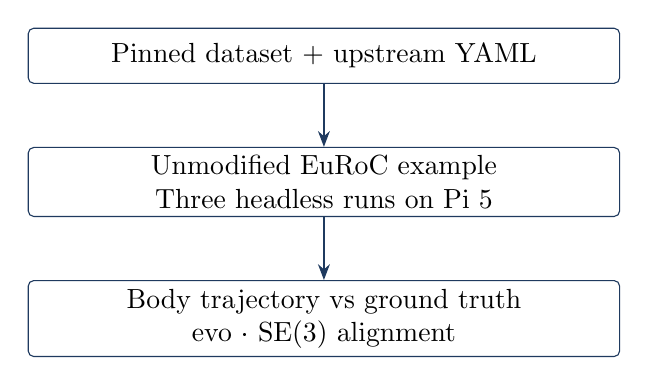
\begin{tikzpicture}[node distance=8mm]
\node[box,text width=73mm,font=\normalsize] (a) {Pinned dataset + upstream YAML};
\node[box,text width=73mm,font=\normalsize,below=of a] (b) {Unmodified EuRoC example\\Three headless runs on Pi 5};
\node[box,text width=73mm,font=\normalsize,below=of b] (c) {Body trajectory vs ground truth\\evo · SE(3) alignment};
\draw[flow](a)--(b);\draw[flow](b)--(c);
\end{tikzpicture}
\end{column}\end{columns}
\vfill\takeaway{Known input separates native-build behavior from D435i acquisition problems.}
\src{N4A/REPORT.md; N4A/provenance.txt}
\note{EuRoC MH_01_easy from official ETH Machine Hall dataset archive. The SDK camera is not involved. Source library has compatibility patches; the stereo_inertial_euroc example, EuRoC.yaml and MH01 timestamps are unchanged. Compare body/IMU exports with body ground truth, after ns-to-s conversion. Association tolerance 0.02 s. Ground truth is laser tracker/motion capture dataset evidence, not a reference collected by this project.}
\end{frame}

% 10
\begin{frame}{N4A result: 0.037--0.042 m translation ATE}
\evidence{MEASURED runs / SOURCE-SUPPORTED paper comparison}
\begin{columns}[T,onlytextwidth]\begin{column}{.38\textwidth}
\begin{tabular}{@{}lr@{}}\toprule
\textbf{Trial} & \textbf{RMSE (m)}\\\midrule
Run 1 & 0.0415\\[6pt]
Run 2 & 0.0368\\[6pt]
Run 3 & 0.0416\\[6pt]
\midrule Mean & 0.040\\[6pt]
Paper MH01 & 0.036\\\bottomrule
\end{tabular}\par\medskip
\small Paper: median of 10 runs.\par
Our three-run median: 0.0415 m.
\end{column}\begin{column}{.58\textwidth}
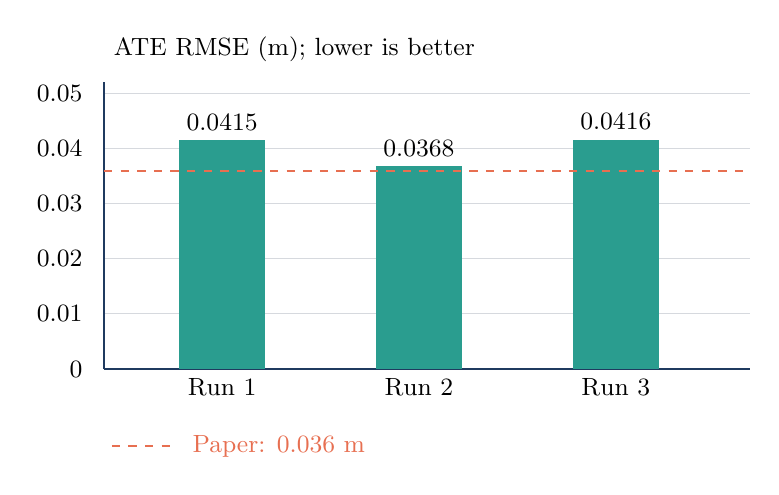
\begin{tikzpicture}[x=1cm,y=70cm,font=\small]
\foreach \v/\l in {0/0,0.01/0.01,0.02/0.02,0.03/0.03,0.04/0.04,0.05/0.05}{\draw[rule](0,\v)--(8.2,\v);\node[anchor=east]at(-.15,\v){\l};}
\draw[navy](0,0)--(8.2,0);\draw[navy](0,0)--(0,.052);
\foreach \x/\v/\l in {1.5/0.0415/Run 1,4/0.0368/Run 2,6.5/0.0416/Run 3}{\fill[teal](\x-.55,0)rectangle(\x+.55,\v);\node[above]at(\x,\v){\v};\node[below]at(\x,0){\l};}
\draw[fault,dashed,thick](0,.036)--(8.2,.036);
\draw[fault,dashed,thick](.1,-.014)--(.9,-.014);
\node[anchor=west,text=fault]at(1,-.014){Paper: 0.036 m};
\node[anchor=west]at(0,.058){ATE RMSE (m); lower is better};
\end{tikzpicture}
\end{column}\end{columns}
\vfill\takeaway{All three runs: IMU initialized, one map, no resets; N4A remains OPEN.}
\src{N4A/eval/ape\_summary.txt; \href{https://arxiv.org/pdf/2007.11898}{Campos et al., 2021, Table II}}
\note{Paper value verified in accepted author manuscript arXiv v2, PDF page 12, Table II, stereo-inertial row, MH01 column. Paper reports median of ten executions. This is similar accuracy on one sequence, not exact statistical reproduction. Local raw RMSE 0.041461, 0.036844, 0.041604 m. Rounded mean 0.040 m. No Sim(3) scale correction is used in these results. Bars start at zero. Under-voltage excludes valid performance timing.}
\end{frame}

% 11
\begin{frame}{N4A supports the native build, with a narrow scope}
\evidence{INFERRED from MEASURED runs / OPEN}
\begin{columns}[T,onlytextwidth]\begin{column}{.48\textwidth}
\begin{block}{Supported on MH01}
\deckitems{\item ARM64 build produces repeat trajectories.
\item Compatibility patches retain similar accuracy.
\item Initialization and map continuity are observed.}
\end{block}
\end{column}\begin{column}{.48\textwidth}
\begin{block}{Still unproven}
\deckitems{\item Sustained D435i delivery on a moving take.
\item Camera--IMU timing and calibration.
\item Real-time speed or robot navigation.}
\end{block}
\end{column}\end{columns}
\vfill\takeaway{Retain the known-data baseline while qualifying each camera-specific input.}
\src{N4A/REPORT.md; Session facts §D}
\note{One sequence and three runs do not prove broad generalization or exact equivalence with the paper. No RPE or wider sequence campaign was reported. Peak RSS 823--828 MiB; this is SLAM runtime memory, distinct from the native compile memory pressure. Wall time includes vocabulary loading and was recorded under power throttling.}
\end{frame}

% 12
\begin{frame}{D435i recording: short tests work; long take failed}
\evidence{MEASURED tests / INFERRED storage bottleneck / OPEN qualification}
\begin{tabular}{@{}L{43mm}L{140mm}@{}}\toprule
\textbf{Take} & \textbf{Observation}\\\midrule
20 s still & Stereo + gyro + accel delivered for 19 s.\newline One $\sim$0.7 s gap in the final second at shutdown.\\[10pt]
100 s hand-moved & Unusable: 0.3--2.9 s gaps after 22 s.\newline Card wrote 16.6 MB/s vs 18.4 MB/s image payload.\\[10pt]
15 s into RAM & IR 29.99 Hz; max gap 33 ms; zero dropped frames.\newline Gyro 200.2 Hz; accel 101 Hz; copied with checksum OK.\\\bottomrule
\end{tabular}
\vfill\takeaway{Record into RAM, then copy: the 100 s RAM take is still unverified.}
\src{14 October addendum §§2--4; smoke\_ram.sh}
\note{Session-reported tests, not new experiments for this deck. Card take: 1.66 GB in 100 s, repeated gaps every roughly 5 s; blocking is a strong inference. No kernel under-voltage or USB errors during this take, but platform power unresolved. RAM test only 15 s. /dev/shm 3.9 GB; 100 s about 1.7 GB is a budget, not a guarantee. N4 stereo profile IR1+IR2 640x480 Y8/30, gyro/200, accel/100, emitter OFF. This does not replace N2 IR1-only 15 Hz or mandatory 300 s soak.}
\end{frame}

% 13
\begin{frame}{Offline replay: first-frame crash; patch 4 awaits rebuild}
\evidence{MEASURED crash / SOURCE-SUPPORTED diagnosis / OPEN verification}
\centering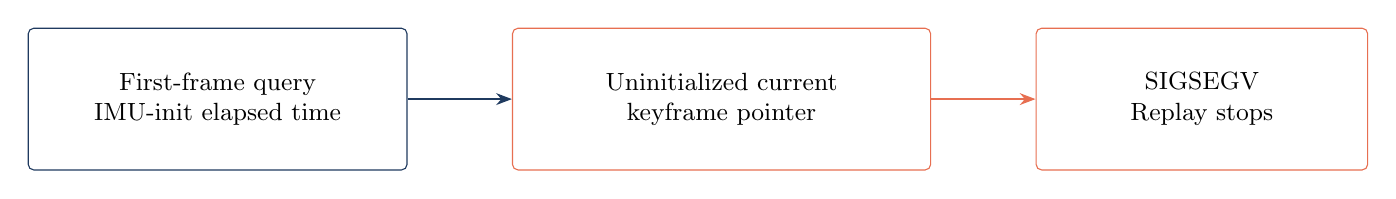
\begin{tikzpicture}[font=\normalsize]
\node[box,text width=46mm,minimum height=18mm] (a) at (0,0) {First-frame query\\IMU-init elapsed time};
\node[box,draw=fault,text width=51mm,minimum height=18mm] (b) at (6.4,0) {Uninitialized current\\keyframe pointer};
\node[box,draw=fault,text width=40mm,minimum height=18mm] (c) at (12.5,0) {SIGSEGV\\Replay stops};
\draw[flow](a)--(b);\draw[faultflow](b)--(c);
\end{tikzpicture}\par\bigskip
\raggedright\textbf{Patch 4:} initialize the pointer to \texttt{nullptr}.\par\medskip
Applied in the Pi build copy; power loss interrupted the rebuild.\par\medskip
Resume build, check linkage, then retry offline replay.
\vfill\takeaway{EuRoC did not call this query; its three-run result is unchanged.}
\src{14 October addendum §5; 15 October lab runbook}
\note{gdb: main → System::GetTimeFromIMUInit → LocalMapping::GetCurrKFTime. LocalMapping::mpCurrentKeyFrame uninitialized: null check reads garbage before first keyframe. Patch: KeyFrame* mpCurrentKeyFrame = nullptr; in include/LocalMapping.h, applied/committed only in Pi build copy. Rebuild stopped after 3 of about 27 library objects. Future command cmake --build build -j4 in ~/orbslam3/ORB_SLAM3; keep logs and verify intended library linkage. No execution or upstream edit for this deck.}
\end{frame}

% 14
\begin{frame}{Blockers: power first, then trustworthy input}
\evidence{MEASURED / ASSUMED / OPEN · 14 October 2026}
{\small\begin{tabular}{@{}L{28mm}L{80mm}L{76mm}@{}}\toprule
\textbf{Risk} & \textbf{Evidence and consequence} & \textbf{What can be done now}\\\midrule
Power / timing & 4 GB Pi: under-voltage in 49\% of samples; timing invalid. 8 GB Pi: under-voltage within 3 min of boot. & \textbf{Unresolved.} Use an adequate 5 A supply; retain power logs for each diagnostic run.\\[5pt]
Storage & 100 s card take dropped frames; RAM test clean for 15 s. USB stick: 1.09 MB/s. & \textbf{Demo workaround:} RAM then checksummed copy. Qualified dataset storage still needed.\\[5pt]
Calibration & Nominal camera--IMU geometry; IMU noise values copied, not measured. & \textbf{OPEN.} Diagnostic room plot has no ground truth; accuracy remains unverified.\\[5pt]
RAM & 8 GB Pi: 7.8 GiB RAM; RAM recording allocation 3.9 GB. & 100 s take $\sim$1.7 GB fits the budget. Recheck free memory; full take unverified.\\\bottomrule
\end{tabular}}
\src{14 October addendum §§1,3,4,6; N4A/REPORT.md and power\_window.log}
\note{14 October addendum §§1,3,4,6 supersedes previous thread findings. No new EuRoC measurement or completed no-swap build is claimed. USB 2.0 stick data untouched. RAM is a bounded diagnostic workaround, not qualified persistent storage. MicroSD stages a copied take; transfer to Mac and verify checksums. Nominal geometry, ASSUMED noise and unknown camera--IMU offset remain. Ethernet loose; 8 GB Pi Wi-Fi unverified (§7).}
\end{frame}

% 15
\begin{frame}{15 October: prepare, rebuild, record into RAM}
\evidence{PLANNED diagnostic demo / OPEN exit criteria}
\begin{tabular}{@{}L{9mm}L{55mm}L{121mm}@{}}\toprule
 & \textbf{Action} & \textbf{Exit evidence}\\\midrule
1 & Set up 8 GB Pi & Adequate power; fixed Pi/cables; secure connection.\newline Fresh N1 $\rightarrow$ N2 $\rightarrow$ N3 evidence; gates stay OPEN.\\[10pt]
2 & Resume patch 4 build & Build exits zero; intended rebuilt library is linked.\newline Retain logs and source/binary hashes.\\[10pt]
3 & Record 100 s into RAM & Smooth early translation + gentle rotation; loop; still ending.\newline Review rates, stamps, gaps, logs and copied-take checksum.\\\bottomrule
\end{tabular}
\vfill\takeaway{Each step starts only when the previous step's exit evidence exists.}
\src{15 October lab runbook; 14 October addendum §§1,4,5,7}
\note{Owner must say CAMERA AVAILABLE before camera or ORB execution. No physical command runs for this build. Camera on blue USB3 port, >=5000M; Pi/connectors stationary. Wi-Fi on 8 GB Pi unverified; match saved host key. N1 → N2 → N3 required; N2 IR1 Y8 640x480/15, gyro/200, accel/100, staged 20 → 105 → mandatory 300 s. Thresholds unchanged: IR 14.25--15.75, gyro 190--210, accel 95--105 Hz; image gap <=0.20 s, motion gap <=0.05 s; positive stamps/steps, no missing frames, clean logs/content/review. Do not put 300 s stereo soak into 3.9 GB RAM. Demo is stereo 30 Hz, 100 s; it does not replace gates. Translate within 1--2 s; 20--30 s varied motion, 10--30 cm all axes, gentle +/-15--30 degree rotations; finish 5--10 s still. Check RAM/card capacity before capture. Acquisition local to Pi; SSH control only.}
\end{frame}

% 16
\begin{frame}{Then: replay, plot, and review before live}
\evidence{PLANNED diagnostic demo / OPEN exit criteria}
\begin{tabular}{@{}L{9mm}L{55mm}L{121mm}@{}}\toprule
 & \textbf{Action} & \textbf{Exit evidence}\\\midrule
4 & Offline replay & Hashed input/settings; initialization; sustained tracking.\newline Review one stable map, resets, queues and nonempty trajectories.\\[10pt]
5 & Plot and review & Copy evidence to Mac; verify checksums; inspect trajectory.\newline Room take has no ground truth: accuracy unverified.\\[10pt]
6 & Live, then summary & Proceed only after offline review; same binary/settings.\newline Retain power/kernel logs, counters and finalized outputs.\\\bottomrule
\end{tabular}
\vfill\takeaway{Nominal-config development runs can inform diagnosis; they cannot qualify VIO.}
\src{15 October lab runbook; 14 October addendum §§5,8}
\note{Offline --bag ... --no-viewer; live omits --bag. Only one process owns camera. Retain warning: IMU Calibration is not available. Geometry nominal, noise ASSUMED, time offset unknown. Tracking state 2 and one map are diagnostic observations, not accuracy acceptance; largest-map export may hide resets. Audit order/domains/IMU bracketing. Offline wall duration/export pose rate do not measure live processing speed. Live needs normal shutdown/finalization and reviewed health/counters. Plot helper matches evo on EuRoC run1, 0.041461 m, a tooling check not room ground truth. Everything remains diagnostic OPEN until power/calibration and gates are evidenced.}
\end{frame}

% 17
\begin{frame}{Summary: baseline retained; camera demo still OPEN}
\evidence{MEASURED progress / OPEN qualification / PLANNED next work}
\Large Three EuRoC runs: 0.037--0.042 m ATE.\par\bigskip
\normalsize\deckitems{
\item Native Pi build is usable on the known-data sequence.
\item Short RAM capture works; 100 s capture remains unverified.
\item Patch 4 rebuild and successful offline replay are pending.
\item Next: RAM take $\rightarrow$ replay $\rightarrow$ plot/review $\rightarrow$ live demo.}
\vfill\takeaway{No gate PASS is claimed. STM32H7 retains balance and motor safety.}
\par\medskip{\small\color{muted}Further detail: course reference deck and learning deck.}
\note{Close the meeting here; four backup slides support questions about alignment, patches, power and storage. Advisor decisions on metric budgets/calibration remain future reviews; no deadline or unsupported request is invented.}
\end{frame}

\appendix
% 18
\begin{frame}{Backup: ATE uses one rigid alignment, without scale}
\evidence{MEASURED evaluation method}
Absolute trajectory error: matched body-position differences after alignment.\par
\[
(R^*,t^*)=\arg\min_{R\in SO(3),\,t}\sum_{i=1}^{n}\|Rp_i+t-q_i\|^2,
\qquad
\mathrm{ATE}_{\mathrm{RMSE}}=\sqrt{\frac{1}{n}\sum_{i=1}^{n}\|R^*p_i+t^*-q_i\|^2}
\]
{\small $p_i$: estimate; $q_i$: ground truth; $n$: matched positions.}\par\medskip
\centering
\begin{tikzpicture}
\node[box,text width=47mm,font=\normalsize] (a) at (0,0) {Body poses\\ns $\rightarrow$ s};
\node[box,text width=48mm,font=\normalsize] (b) at (6.2,0) {Associate to GT\\Tolerance 0.02 s};
\node[box,text width=48mm,font=\normalsize] (c) at (12.4,0) {Align SE(3)\\Position RMSE};
\draw[flow](a)--(b);\draw[flow](b)--(c);
\end{tikzpicture}\par\bigskip
\raggedright\texttt{evo\_ape tum gt.tum est.tum -a --t\_max\_diff 0.02}
\vfill\takeaway{Stereo-inertial has metric scale; Sim(3) would answer a different question.}
\src{N4A/REPORT.md; N4A/eval/ape\_summary.txt}
\note{p_i estimate, q_i associated ground truth; both body positions. R and t are one global alignment, not local per-segment fits. n is associated pose count; retained exports have 3678 poses, but associated count is not re-invented. Translation ATE is in metres. RPE, alignment residuals, coverage exclusions and full metric campaign remain incomplete.}
\end{frame}

% 19
\begin{frame}{Backup: three build patches; patch 4 rebuild pending}
\evidence{MEASURED build / INFERRED consistency / OPEN patch 4 rebuild}
\begin{tabular}{@{}L{53mm}L{128mm}@{}}\toprule
\textbf{Patch} & \textbf{Reason / limit}\\\midrule
C++17; remove\newline\texttt{-march=native} & Pangolin 0.9.1 / Ubuntu 24.04 toolchain compatibility.\newline Compile configuration changed; retain source and binary hashes.\\[8pt]
Sophus tests OFF & GCC 13 aarch64 array-bounds warning fails their \texttt{-Werror}.\newline ORB-SLAM3 uses Sophus headers; disabled tests are not validated.\\[8pt]
\texttt{mnFullBAIdx++}\newline$\rightarrow$ \texttt{= true} & C++17 forbids incrementing bool.\newline Preserves the prior C++11 bool-increment effect.\\[8pt]
Current keyframe $\rightarrow$ \texttt{nullptr} & Patch 4 avoids the first-frame uninitialized-pointer query.\newline Applied in Pi copy; rebuild and replay unverified.\\\bottomrule
\end{tabular}
\vfill\takeaway{MH01 accuracy is evidence for this build; it does not validate every code path.}
\src{Session facts §C; Pi build/build\_orbslam3.sh; N4A/provenance.txt; 14 October addendum §5}
\note{Upstream 4452a3c4ab75b1cde34e5505a36ec3f9edcdc4c4. Build copied into ~/orbslam3/ORB_SLAM3, repo checkout preserved. Full build logs/patches are partly Pi-side, as documented in the session facts; do not imply all raw logs are on the Mac. Example and EuRoC configuration remained upstream. Addendum §5: patch 4 in include/LocalMapping.h; rebuild interrupted by power loss. No fresh build or source mutation occurred for this deck.}
\end{frame}

% 20
\begin{frame}{Backup: live power faults in 87 of 178 samples}
\evidence{MEASURED samples / CALCULATED 48.9\%}
\centering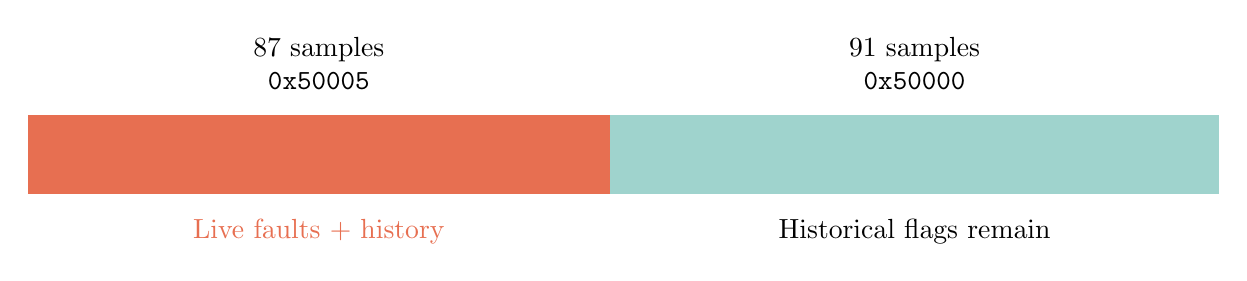
\begin{tikzpicture}[font=\normalsize,x=.085cm]
\fill[fault](0,0)rectangle(87,1);
\fill[teal!45](87,0)rectangle(178,1);
\node[above,align=center]at(43.5,1.2){87 samples\\\texttt{0x50005}};
\node[above,align=center]at(132.5,1.2){91 samples\\\texttt{0x50000}};
\node[below,align=center,text=fault]at(43.5,-.2){Live faults + history};
\node[below,align=center]at(132.5,-.2){Historical flags remain};
\end{tikzpicture}\par\bigskip
\raggedright 5-second sampling during the EuRoC runs.\par\medskip
Maximum observed temperature: about 63\,$^{\circ}$C.\par\medskip
Pi UTC labels were about 80 minutes behind; NTP corrected later.
\vfill\takeaway{Historical-only flags are not a clean N0 result; timing must be repeated.}
\src{N4A/power\_window.log; N4A/REPORT.md clock note}
\note{0x50005 records live under-voltage and throttling plus historical bits; 0x50000 retains the historical bits. No claim about exact duty cycle between samples. Maximum logged temperature 63.1 C. Build had 46 events per session summary, separate from this run sample denominator. Clock offset affects cross-machine UTC correlation; within-run elapsed durations have no observed clock step, but wall time includes vocabulary load and is not per-frame compute.}
\end{frame}

% 21
\begin{frame}{Backup: stereo payload already consumes the old write margin}
\evidence{CALCULATED payload / MEASURED tests / OPEN storage}
\[
640\times480\times1\times2\times30
=18{,}432{,}000\ \mathrm{B/s}
\approx18.4\ \mathrm{MB/s}
\]
\begin{tabular}{@{}L{62mm}L{119mm}@{}}\toprule
\textbf{Quantity} & \textbf{Implication}\\\midrule
100 s stereo payload & 1.84 GB before overhead; failed take wrote 1.66 GB.\\[10pt]
100 s card take: 16.6 MB/s & Repeated gaps; microSD blocking strongly inferred.\\[10pt]
RAM: 3.9 GB allocation & 15 s test clean; 100 s $\sim$1.7 GB budget remains unverified.\\[10pt]
USB stick: 1.09 MB/s & Too slow for recording; qualified dataset storage still needed.\\\bottomrule
\end{tabular}
\vfill\takeaway{Qualify storage under load and copy takes to the Mac after each session.}
\src{14 October addendum §§3,4,6; stereo payload calculation}
\note{Decimal units: MB=10^6 B, GB=10^9 B. Calculations include only two Y8 image planes, not IMU, metadata, SQLite/container overhead, filesystem or headroom. 100 s image payload 1.8432 GB; failed 1.66 GB take and 1.7 GB RAM budget are not proof of full-frame delivery. Recheck retained counts and capacity. V30/A2 card ordered, not received/qualified. MicroSD policy remains OS/tools/small logs; large captures require separately qualified storage. Preserve historical logs; proposed card clone and migration are not executed here.}
\end{frame}
\begin{frame}{References}
\small
C. Campos, R. Elvira, J. J. G\'omez Rodr\'iguez, J. M. M. Montiel, J. D. Tard\'os. ORB-SLAM3: An accurate open-source library for visual, visual--inertial and multi-map SLAM. \emph{IEEE Transactions on Robotics}, 37(6), 2021. \href{https://arxiv.org/abs/2007.11898}{arXiv:2007.11898}\par\medskip
M. Burri et al. The EuRoC micro aerial vehicle datasets. \emph{International Journal of Robotics Research}, 35(10), 2016.\par\medskip
Project evidence (experiment reports, logs and trajectories) is listed per slide in the speaker notes.
\end{frame}
\end{document}
